\documentclass[12pt]{article}

\usepackage[top=50pt, bottom=50pt, left=90pt, right=90pt]{geometry}
\usepackage[pdftex]{graphicx}

\usepackage{lipsum}%% a garbage package you don't need except to create examples.
\usepackage{fancyhdr}
\pagestyle{fancy}

%This is some header and footer information
\lfoot{Kids Coding Club}
\rfoot{\thepage}
\cfoot{}
\renewcommand{\headrulewidth}{0pt}
\renewcommand{\footrulewidth}{0.4pt}

%Basic title information about original author and title
\title{Class 1 - Introduction to Coding}
\author{Chris Hight}
\date{\today}
 
 
%This is where we start the document
\begin{document}
\maketitle

\section*{Pre-Class Setup}
	\begin{itemize}
		
		\item Browser 1 - Private tabs
		\begin{itemize}
			\item Tab 1 - Scratch login page
			\item Tab 2 - Dragon Chase program
		\end{itemize}
		
		\item Browser 2
		\begin{itemize}
			\item 3 Scratch Projects
		\end{itemize} 
		
	\end{itemize}




\section*{Introduction}

\subsection*{Introduce Program Goal}
	\begin{itemize}
		\item We are here to introduce a sustainable and understandable code experience.
		\item We are teaching to encourage creativity and thinking different.
		\begin{itemize}
			\item Because we want to foster creativity our projects are a guideline not a requirement but we want everybody working on projects during the free time and not playing games.
		\end{itemize}
		\item We are here to teach to all ages
		\begin{itemize}
			\item We would like the parents to obtain knowledge as well so that we are growing not just a single new computer scientist but a family of them.
		\end{itemize}
		\item The first four weeks there will be 3 projects provided, we recommend picking one to focus on though all three projects will be available for review.
		\item The first hour of the class will have lecture teaching the basics of code, how it behaves and how we can use it!
		\item During the second hour of class the kids will work on projects
		\item This changes during the second four weeks where we will learn electrical engineering and coding during the first hour
		\item During the second hour of the last four weeks we will slowly program a sumo bot to perform different actions.
	\end{itemize}



\subsection*{Introduce Teachers}
	\begin{itemize}
		\item Have teachers introduce themselves to the group with topics like:
		\begin{itemize}
			\item Their name
			\item Experience / Specialty
			\item Fun facts about themselves / Hobbies / interests
		\end{itemize}
	\end{itemize}



\subsection*{What is coding?}
	\begin{itemize}
		\item Coding is a way for humans to tell computers how to behave and respond to user input.
		\item It is a list of tasks that the computer can understand.
		\item Its becoming a very important skill to learn, it is used by many occupations such as:
		\begin{itemize}
			\item Computer Scientists
			\item Web Developers
			\item Electrical Engineers
			\item Scientists (Anthropologists, biologists, chemists…)
			\item Engineers
			\item and many other careers that most don't consider (accountants, civil engineers…)
		\end{itemize}
	\end{itemize}



\subsection*{What is a program?}
	\begin{itemize}
		\item We take the small instructions that we make with code and we write that code into programs to tell the computer what to do.
		\item Programs are like a recipe, just like a recipe for baking a cake or making a pizza!
		\item There has to be a logical order otherwise our program will break. 
		\item We can make a program to bake a cake:  (show instructions english and java type program)
		\begin{itemize}
			\item Preheat the oven to 350 ℉  - oven.preheat(350, “F”)
			\item Grease cake pan - pan.grease( );
			\item Mix cake mix, eggs, water
			\item pour mix into bowl
			\item Bake
		\end{itemize}
		\item If we break the logical sequence, what if we forget to preheat the oven?!
		\item The computer doesn't know how to handle the instructions we write.  These instructions are converted to 1s and 0s so that the computer knows what to do with them
		\item What do real programs do/control
		\begin{itemize}
			\item Video games! These are solving lots and lots of math equations, sometimes around 1000 per second
			\item Appliances (toasters, dishwasher, ovens…)
			\item Cars
		\end{itemize}
	\end{itemize}



\subsection*{What is Scratch?}
	\begin{itemize}
		\item Why are we using scratch?
		\begin{itemize}
			\item It's Free!
			\item Local schools and organizations are teaching scratch and other visual coding languages
			\item There are plenty of websites such as code.org that also use visual coding so this is a very transferable skill to play with other systems
			\item Everybody can have their own account so they can save their projects and work on them elsewhere.
		\end{itemize}
		\item How is it effective?
		\begin{itemize}
			\item Scratch blocks are pre written blocks of code that allow beginners to focus on how a program and logic works and worry less about remembering the syntax of a language.
			\item It's easy to see how a program works, it's very easy to read and write.
			\item Allows for easy experimentation, if you break your program it is easy to put back together.
			\item Once you learn how languages work, its easy to learn new languages.
		\end{itemize}
	\end{itemize}






\section*{Dragon Chase}

\subsection*{Move the Cat - Cat Sprite}
	\begin{itemize}
		\item Let’s make the cat face towards the mouse pointer first
		\begin{center}
			\item[] 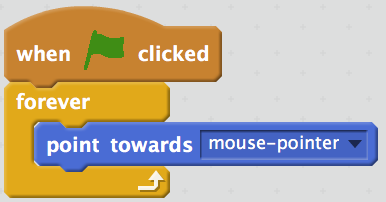
\includegraphics[scale=1.0]{./Images/dragon1.png}
		\end{center}
		\newpage
		\item Now we can make the cat move forward towards the mouse
		\begin{center}
			\item[] 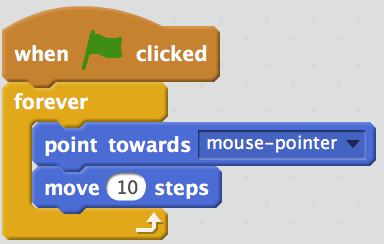
\includegraphics[scale=1.0]{./Images/dragon2.png}
		\end{center}
		\item Add a backdrop to help show that the cat is moving
		\begin{center}
			\item[] 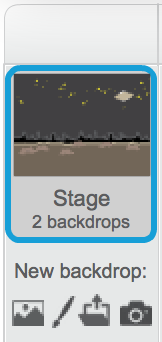
\includegraphics[scale=1.0]{./Images/dragon3.png}
		\end{center}
	\end{itemize}
	
	
	
\subsection*{Adding the Dragon - Dragon Sprite}
	\begin{itemize}
		\item First let’s make the dragon face towards the cat
		\begin{center}
			\item[] 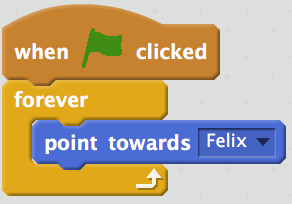
\includegraphics[scale=1.0]{./Images/dragon4.png}
		\end{center}
		\newpage
		\item To make the dragon chase the cat we add a movement block
		\begin{center}
			\item[] 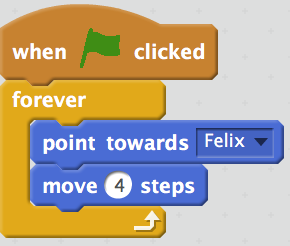
\includegraphics[scale=1.0]{./Images/dragon5.png}
		\end{center}
		\item We want to give the cat a head start so we set the dragons starting point slightly off of the screen. We will also reset the dragons image to default.
		\begin{center}
			\item[] 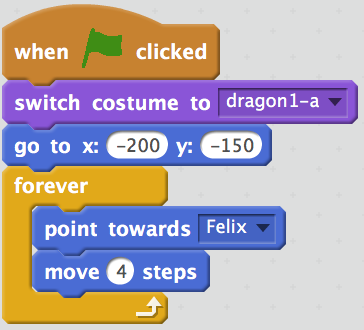
\includegraphics[scale=1.0]{./Images/dragon6.png}
		\end{center}
	\end{itemize}
	
	
	
\subsection*{Ending the Game - Dragon Sprite}
	\begin{itemize}
		\item The dragon will need to end the game when he has caught the cat.  We start by adding a control block called wait, we will add a sensing block to target the cat.
		\begin{center}
			\item[] 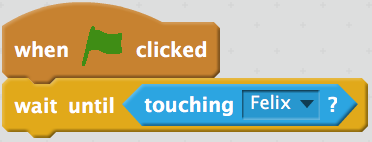
\includegraphics[scale=1.0]{./Images/dragon7.png}
		\end{center}
		\newpage
		\item We have to show that the dragon has caught the cat.  The dragon has a second sprite that is him shooting fire. We will use a switch costume block.
		\begin{center}
			\item[] 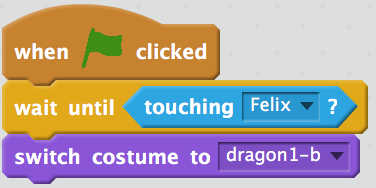
\includegraphics[scale=1.0]{./Images/dragon8.png}
		\end{center}
		\item We need to end the program now. There is a special block for this.
		\begin{center}
			\item[] 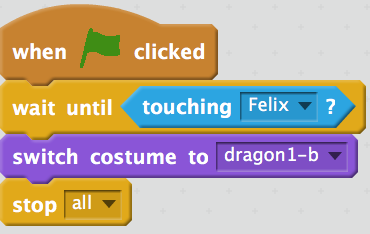
\includegraphics[scale=1.0]{./Images/dragon9.png}
		\end{center}
	\end{itemize}
	
	
	
\subsection*{Time Scoring - Dragon or Cat Sprite}
	\begin{itemize}
		\item We are going to score the game based on how long the cat stays away from the dragon.  We need to make a new variable called time.
		\begin{center}
			\item[] 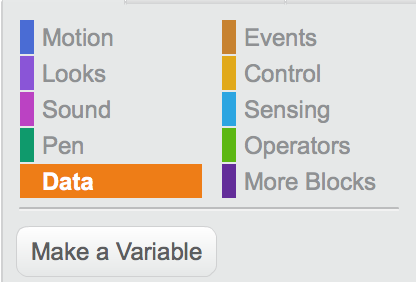
\includegraphics[scale=.80]{./Images/dragon10.png}
		\end{center}
		\newpage
		\item When we name the variable, we want to make it available to all sprites.
		\begin{center}
			\item[] 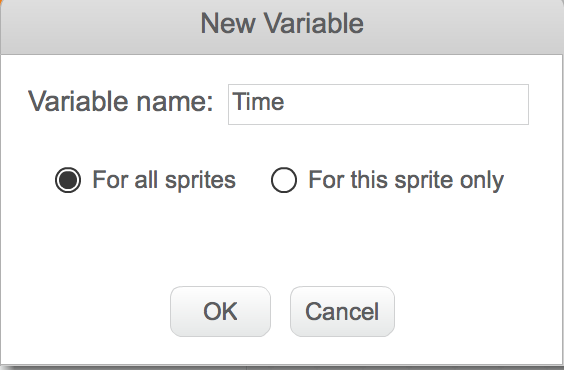
\includegraphics[scale=.80]{./Images/dragon11.png}
		\end{center}
		\item There will be new blocks in the data section now.
		\begin{center}
			\item[] 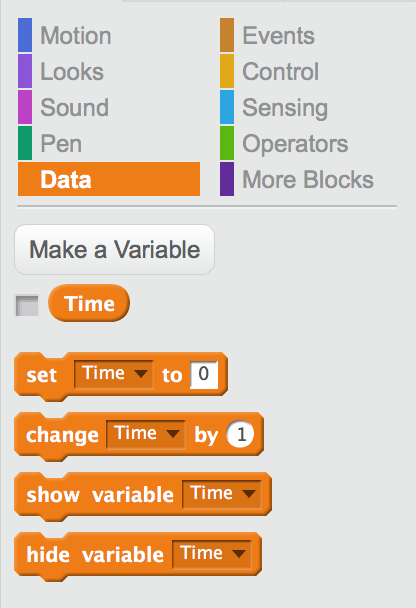
\includegraphics[scale=.80]{./Images/dragon12.png}
		\end{center}
		\item When the program starts, we need to set the time variable to zero so that our score resets.
		\begin{center}
			\item[] 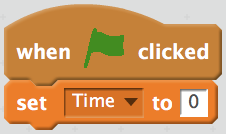
\includegraphics[scale=.50]{./Images/dragon13.png}
		\end{center}
		\newpage
		\item While our program is running we want time to increase continually. We can use a data block to increment time.
		\begin{center}
			\item[] 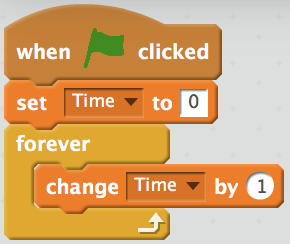
\includegraphics[scale=.50]{./Images/dragon14.png}
		\end{center}
		\item With the last block we see that its counting faster than 1 tick per second. We need to add a delay so that it only increases every second.
		\begin{center}
			\item[] 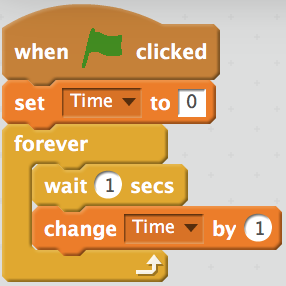
\includegraphics[scale=.50]{./Images/dragon15}
		\end{center}
	\end{itemize}

\end{document}




